\documentclass{standalone}
\usepackage{tikz}
\usetikzlibrary{patterns, positioning}

\begin{document}
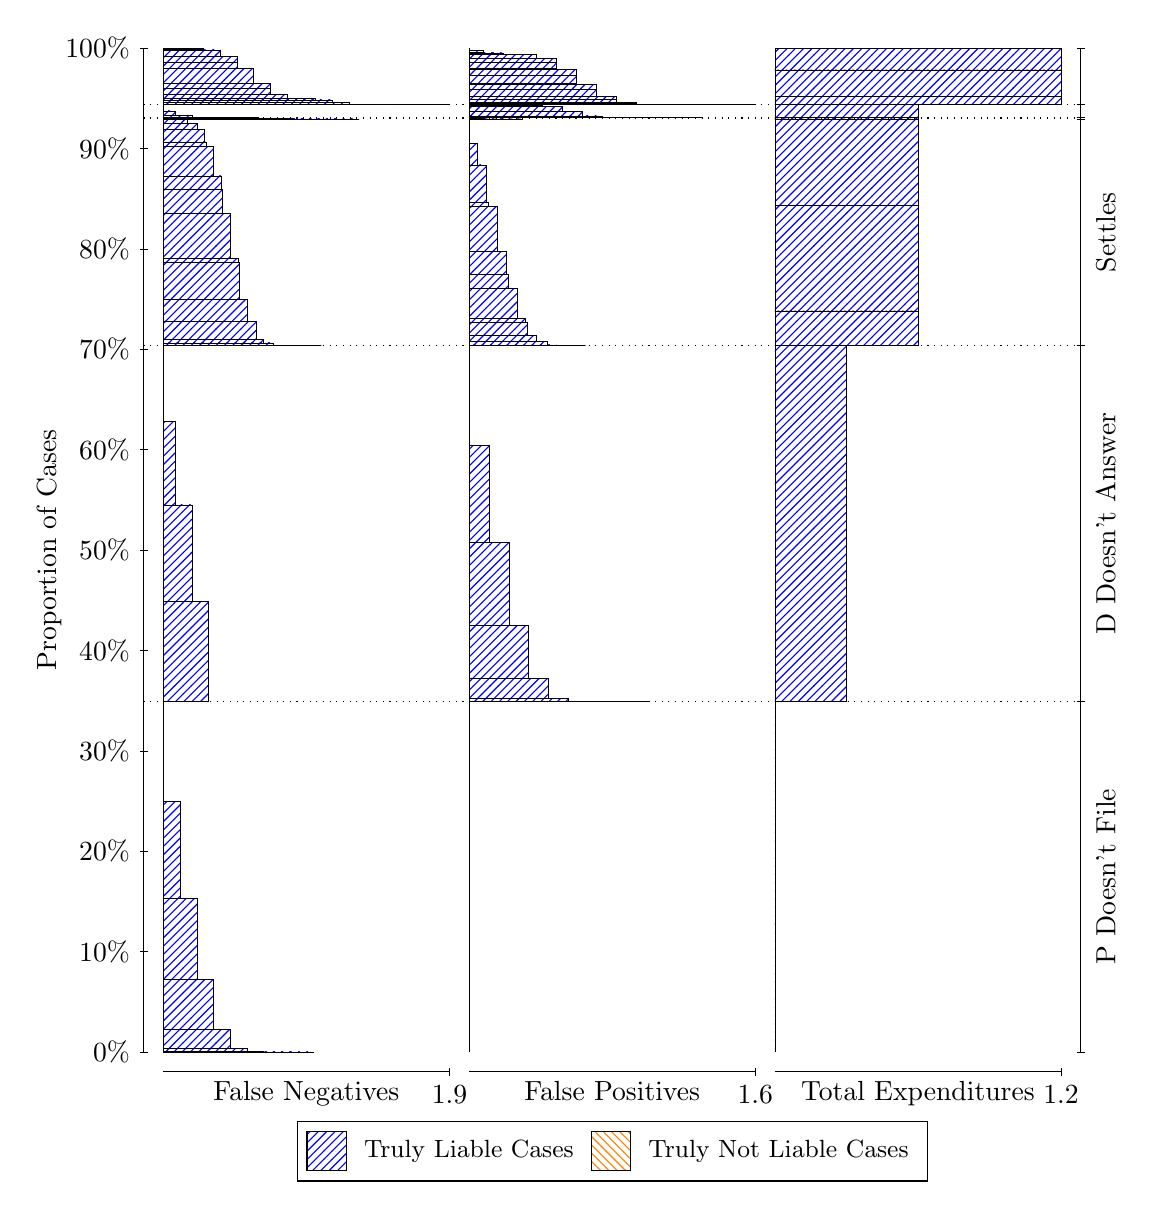
\begin{tikzpicture}
\draw[black, very thin] (1.5,1.75) -- (1.5,14.5);
\node[rotate=90, anchor=center] at (0.3, 8.125) {Proportion of Cases};
\draw[black, very thin] (1.45,1.75) -- (1.55,1.75);
\node[anchor=east] at (1.45, 1.75) {0\%};
\draw[black, very thin] (1.45,3.025) -- (1.55,3.025);
\node[anchor=east] at (1.45, 3.025) {10\%};
\draw[black, very thin] (1.45,4.3) -- (1.55,4.3);
\node[anchor=east] at (1.45, 4.3) {20\%};
\draw[black, very thin] (1.45,5.575) -- (1.55,5.575);
\node[anchor=east] at (1.45, 5.575) {30\%};
\draw[black, very thin] (1.45,6.85) -- (1.55,6.85);
\node[anchor=east] at (1.45, 6.85) {40\%};
\draw[black, very thin] (1.45,8.125) -- (1.55,8.125);
\node[anchor=east] at (1.45, 8.125) {50\%};
\draw[black, very thin] (1.45,9.4) -- (1.55,9.4);
\node[anchor=east] at (1.45, 9.4) {60\%};
\draw[black, very thin] (1.45,10.675) -- (1.55,10.675);
\node[anchor=east] at (1.45, 10.675) {70\%};
\draw[black, very thin] (1.45,11.95) -- (1.55,11.95);
\node[anchor=east] at (1.45, 11.95) {80\%};
\draw[black, very thin] (1.45,13.225) -- (1.55,13.225);
\node[anchor=east] at (1.45, 13.225) {90\%};
\draw[black, very thin] (1.45,14.5) -- (1.55,14.5);
\node[anchor=east] at (1.45, 14.5) {100\%};

\draw[black, very thin] (13.4,1.75) -- (13.4,14.5);
\draw[black, very thin] (13.35,1.75) -- (13.45,1.75);
\node[anchor=west] at (13.35, 1.75) {};
\draw[black, very thin] (13.35,6.1976) -- (13.45,6.1976);
\node[anchor=west] at (13.35, 6.1976) {};
\draw[black, very thin] (13.35,10.72) -- (13.45,10.72);
\node[anchor=west] at (13.35, 10.72) {};
\draw[black, very thin] (13.35,13.601) -- (13.45,13.601);
\node[anchor=west] at (13.35, 13.601) {};
\draw[black, very thin] (13.35,13.62) -- (13.45,13.62);
\node[anchor=west] at (13.35, 13.62) {};
\draw[black, very thin] (13.35,13.78) -- (13.45,13.78);
\node[anchor=west] at (13.35, 13.78) {};
\draw[black, very thin] (13.35,14.5) -- (13.45,14.5);
\node[anchor=west] at (13.35, 14.5) {};

\draw[black, very thin, pattern color=blue, pattern=north east lines] (1.75,1.75) rectangle (3.6623,1.75);
\draw[black, very thin, pattern color=blue, pattern=north east lines] (1.75,1.75) rectangle (3.4498,1.75);
\draw[black, very thin, pattern color=blue, pattern=north east lines] (1.75,1.75) rectangle (3.2373,1.7502);
\draw[black, very thin, pattern color=blue, pattern=north east lines] (1.75,1.7502) rectangle (3.0249,1.7542);
\draw[black, very thin, pattern color=blue, pattern=north east lines] (1.75,1.7542) rectangle (2.8124,1.8003);
\draw[black, very thin, pattern color=blue, pattern=north east lines] (1.75,1.8003) rectangle (2.5999,2.0376);
\draw[black, very thin, pattern color=blue, pattern=north east lines] (1.75,2.0376) rectangle (2.3874,2.6718);
\draw[black, very thin, pattern color=blue, pattern=north east lines] (1.75,2.6718) rectangle (2.175,3.7041);
\draw[black, very thin, pattern color=blue, pattern=north east lines] (1.75,3.7041) rectangle (1.9625,4.9286);
\draw[black, very thin, pattern color=orange, pattern=north west lines] (1.75,4.9286) rectangle (1.75,4.9286);
\draw[black, very thin, pattern color=blue, pattern=north east lines] (1.75,4.9286) rectangle (1.75,6.1976);
\draw[black, very thin, pattern color=blue, pattern=north east lines] (1.75,6.1976) rectangle (2.3237,7.4675);
\draw[black, very thin, pattern color=blue, pattern=north east lines] (1.75,7.4675) rectangle (2.1112,8.6984);
\draw[black, very thin, pattern color=blue, pattern=north east lines] (1.75,8.6984) rectangle (1.8987,9.7542);
\draw[black, very thin, pattern color=orange, pattern=north west lines] (1.75,9.7542) rectangle (1.75,9.7542);
\draw[black, very thin, pattern color=blue, pattern=north east lines] (1.75,9.7542) rectangle (1.75,10.72);
\draw[black, very thin, pattern color=blue, pattern=north east lines] (1.75,10.72) rectangle (3.7579,10.72);
\draw[black, very thin, pattern color=blue, pattern=north east lines] (1.75,10.72) rectangle (3.6623,10.72);
\draw[black, very thin, pattern color=blue, pattern=north east lines] (1.75,10.72) rectangle (3.5667,10.72);
\draw[black, very thin, pattern color=blue, pattern=north east lines] (1.75,10.72) rectangle (3.5454,10.72);
\draw[black, very thin, pattern color=blue, pattern=north east lines] (1.75,10.72) rectangle (3.4498,10.72);
\draw[black, very thin, pattern color=blue, pattern=north east lines] (1.75,10.72) rectangle (3.3542,10.721);
\draw[black, very thin, pattern color=blue, pattern=north east lines] (1.75,10.721) rectangle (3.3329,10.721);
\draw[black, very thin, pattern color=blue, pattern=north east lines] (1.75,10.721) rectangle (3.2373,10.722);
\draw[black, very thin, pattern color=blue, pattern=north east lines] (1.75,10.722) rectangle (3.1417,10.756);
\draw[black, very thin, pattern color=blue, pattern=north east lines] (1.75,10.756) rectangle (3.1205,10.756);
\draw[black, very thin, pattern color=blue, pattern=north east lines] (1.75,10.756) rectangle (3.0249,10.795);
\draw[black, very thin, pattern color=blue, pattern=north east lines] (1.75,10.795) rectangle (2.9292,11.029);
\draw[black, very thin, pattern color=blue, pattern=north east lines] (1.75,11.029) rectangle (2.908,11.031);
\draw[black, very thin, pattern color=blue, pattern=north east lines] (1.75,11.031) rectangle (2.8124,11.305);
\draw[black, very thin, pattern color=blue, pattern=north east lines] (1.75,11.305) rectangle (2.7168,11.782);
\draw[black, very thin, pattern color=blue, pattern=north east lines] (1.75,11.782) rectangle (2.6955,11.829);
\draw[black, very thin, pattern color=blue, pattern=north east lines] (1.75,11.829) rectangle (2.5999,12.4);
\draw[black, very thin, pattern color=blue, pattern=north east lines] (1.75,12.4) rectangle (2.5043,12.7);
\draw[black, very thin, pattern color=blue, pattern=north east lines] (1.75,12.7) rectangle (2.483,12.876);
\draw[black, very thin, pattern color=blue, pattern=north east lines] (1.75,12.876) rectangle (2.3874,13.253);
\draw[black, very thin, pattern color=blue, pattern=north east lines] (1.75,13.253) rectangle (2.2918,13.308);
\draw[black, very thin, pattern color=blue, pattern=north east lines] (1.75,13.308) rectangle (2.2706,13.471);
\draw[black, very thin, pattern color=blue, pattern=north east lines] (1.75,13.471) rectangle (2.175,13.542);
\draw[black, very thin, pattern color=blue, pattern=north east lines] (1.75,13.542) rectangle (2.0793,13.545);
\draw[black, very thin, pattern color=blue, pattern=north east lines] (1.75,13.545) rectangle (2.0581,13.591);
\draw[black, very thin, pattern color=blue, pattern=north east lines] (1.75,13.591) rectangle (1.9625,13.595);
\draw[black, very thin, pattern color=blue, pattern=north east lines] (1.75,13.595) rectangle (1.8669,13.595);
\draw[black, very thin, pattern color=blue, pattern=north east lines] (1.75,13.595) rectangle (1.8456,13.601);
\draw[black, very thin, pattern color=orange, pattern=north west lines] (1.75,13.601) rectangle (1.75,13.601);
\draw[black, very thin, pattern color=blue, pattern=north east lines] (1.75,13.601) rectangle (1.75,13.601);
\draw[black, very thin, pattern color=blue, pattern=north east lines] (1.75,13.601) rectangle (4.236,13.601);
\draw[black, very thin, pattern color=blue, pattern=north east lines] (1.75,13.601) rectangle (4.0235,13.601);
\draw[black, very thin, pattern color=blue, pattern=north east lines] (1.75,13.601) rectangle (3.811,13.601);
\draw[black, very thin, pattern color=blue, pattern=north east lines] (1.75,13.601) rectangle (3.5985,13.601);
\draw[black, very thin, pattern color=blue, pattern=north east lines] (1.75,13.601) rectangle (3.3861,13.602);
\draw[black, very thin, pattern color=blue, pattern=north east lines] (1.75,13.602) rectangle (3.1736,13.61);
\draw[black, very thin, pattern color=blue, pattern=north east lines] (1.75,13.61) rectangle (2.9611,13.618);
\draw[black, very thin, pattern color=blue, pattern=north east lines] (1.75,13.618) rectangle (2.7486,13.62);
\draw[black, very thin, pattern color=blue, pattern=north east lines] (1.75,13.62) rectangle (2.5362,13.62);
\draw[black, very thin, pattern color=blue, pattern=north east lines] (1.75,13.62) rectangle (2.3237,13.62);
\draw[black, very thin, pattern color=orange, pattern=north west lines] (1.75,13.62) rectangle (1.75,13.62);
\draw[black, very thin, pattern color=blue, pattern=north east lines] (1.75,13.62) rectangle (2.3237,13.623);
\draw[black, very thin, pattern color=blue, pattern=north east lines] (1.75,13.623) rectangle (2.1112,13.642);
\draw[black, very thin, pattern color=blue, pattern=north east lines] (1.75,13.642) rectangle (1.8987,13.702);
\draw[black, very thin, pattern color=orange, pattern=north west lines] (1.75,13.702) rectangle (1.75,13.702);
\draw[black, very thin, pattern color=blue, pattern=north east lines] (1.75,13.702) rectangle (1.75,13.78);
\draw[black, very thin, pattern color=blue, pattern=north east lines] (1.75,13.78) rectangle (5.3833,13.78);
\draw[black, very thin, pattern color=blue, pattern=north east lines] (1.75,13.78) rectangle (5.1709,13.78);
\draw[black, very thin, pattern color=blue, pattern=north east lines] (1.75,13.78) rectangle (4.9584,13.78);
\draw[black, very thin, pattern color=blue, pattern=north east lines] (1.75,13.78) rectangle (4.7459,13.78);
\draw[black, very thin, pattern color=blue, pattern=north east lines] (1.75,13.78) rectangle (4.7459,13.78);
\draw[black, very thin, pattern color=blue, pattern=north east lines] (1.75,13.78) rectangle (4.5334,13.781);
\draw[black, very thin, pattern color=blue, pattern=north east lines] (1.75,13.781) rectangle (4.5334,13.781);
\draw[black, very thin, pattern color=blue, pattern=north east lines] (1.75,13.781) rectangle (4.321,13.782);
\draw[black, very thin, pattern color=blue, pattern=north east lines] (1.75,13.782) rectangle (4.321,13.787);
\draw[black, very thin, pattern color=blue, pattern=north east lines] (1.75,13.787) rectangle (4.1722,13.787);
\draw[black, very thin, pattern color=blue, pattern=north east lines] (1.75,13.787) rectangle (4.1085,13.805);
\draw[black, very thin, pattern color=blue, pattern=north east lines] (1.75,13.805) rectangle (4.1085,13.808);
\draw[black, very thin, pattern color=blue, pattern=north east lines] (1.75,13.808) rectangle (3.9597,13.808);
\draw[black, very thin, pattern color=blue, pattern=north east lines] (1.75,13.808) rectangle (3.896,13.839);
\draw[black, very thin, pattern color=blue, pattern=north east lines] (1.75,13.839) rectangle (3.896,13.841);
\draw[black, very thin, pattern color=blue, pattern=north east lines] (1.75,13.841) rectangle (3.7473,13.841);
\draw[black, very thin, pattern color=blue, pattern=north east lines] (1.75,13.841) rectangle (3.7473,13.842);
\draw[black, very thin, pattern color=blue, pattern=north east lines] (1.75,13.842) rectangle (3.6835,13.857);
\draw[black, very thin, pattern color=blue, pattern=north east lines] (1.75,13.857) rectangle (3.5348,13.862);
\draw[black, very thin, pattern color=blue, pattern=north east lines] (1.75,13.862) rectangle (3.5348,13.863);
\draw[black, very thin, pattern color=blue, pattern=north east lines] (1.75,13.863) rectangle (3.4711,13.865);
\draw[black, very thin, pattern color=blue, pattern=north east lines] (1.75,13.865) rectangle (3.3223,13.914);
\draw[black, very thin, pattern color=blue, pattern=north east lines] (1.75,13.914) rectangle (3.2586,13.914);
\draw[black, very thin, pattern color=blue, pattern=north east lines] (1.75,13.914) rectangle (3.2586,13.914);
\draw[black, very thin, pattern color=blue, pattern=north east lines] (1.75,13.914) rectangle (3.1098,13.986);
\draw[black, very thin, pattern color=blue, pattern=north east lines] (1.75,13.986) rectangle (3.1098,14.053);
\draw[black, very thin, pattern color=blue, pattern=north east lines] (1.75,14.053) rectangle (3.0461,14.053);
\draw[black, very thin, pattern color=blue, pattern=north east lines] (1.75,14.053) rectangle (3.0461,14.053);
\draw[black, very thin, pattern color=blue, pattern=north east lines] (1.75,14.053) rectangle (2.8974,14.243);
\draw[black, very thin, pattern color=blue, pattern=north east lines] (1.75,14.243) rectangle (2.8336,14.243);
\draw[black, very thin, pattern color=blue, pattern=north east lines] (1.75,14.243) rectangle (2.6849,14.315);
\draw[black, very thin, pattern color=blue, pattern=north east lines] (1.75,14.315) rectangle (2.6849,14.32);
\draw[black, very thin, pattern color=blue, pattern=north east lines] (1.75,14.32) rectangle (2.6849,14.398);
\draw[black, very thin, pattern color=blue, pattern=north east lines] (1.75,14.398) rectangle (2.4724,14.473);
\draw[black, very thin, pattern color=blue, pattern=north east lines] (1.75,14.473) rectangle (2.4724,14.476);
\draw[black, very thin, pattern color=blue, pattern=north east lines] (1.75,14.476) rectangle (2.2599,14.483);
\draw[black, very thin, pattern color=blue, pattern=north east lines] (1.75,14.483) rectangle (2.2599,14.484);
\draw[black, very thin, pattern color=blue, pattern=north east lines] (1.75,14.484) rectangle (2.2599,14.497);
\draw[black, very thin, pattern color=blue, pattern=north east lines] (1.75,14.497) rectangle (2.0475,14.5);
\draw[black, very thin, pattern color=blue, pattern=north east lines] (1.75,14.5) rectangle (2.0475,14.5);
\draw[black, very thin, pattern color=blue, pattern=north east lines] (1.75,14.5) rectangle (1.835,14.5);
\draw[black, very thin, pattern color=blue, pattern=north east lines] (1.75,14.5) rectangle (1.835,14.5);
\draw[black, very thin, pattern color=orange, pattern=north west lines] (1.75,14.5) rectangle (1.75,14.5);
\draw[black, very thin, pattern color=blue, pattern=north east lines] (1.75,14.5) rectangle (1.75,14.5);
\draw[black, very thin, pattern color=orange, pattern=north west lines] (5.6333,1.75) rectangle (5.6333,1.75);
\draw[black, very thin, pattern color=blue, pattern=north east lines] (5.6333,1.75) rectangle (5.6333,6.1976);
\draw[black, very thin, pattern color=orange, pattern=north west lines] (5.6333,6.1976) rectangle (7.9042,6.1976);
\draw[black, very thin, pattern color=blue, pattern=north east lines] (5.6333,6.1976) rectangle (7.9042,6.1976);
\draw[black, very thin, pattern color=blue, pattern=north east lines] (5.6333,6.1976) rectangle (7.6519,6.1976);
\draw[black, very thin, pattern color=blue, pattern=north east lines] (5.6333,6.1976) rectangle (7.3995,6.1977);
\draw[black, very thin, pattern color=blue, pattern=north east lines] (5.6333,6.1977) rectangle (7.1472,6.2);
\draw[black, very thin, pattern color=blue, pattern=north east lines] (5.6333,6.2) rectangle (6.8949,6.2423);
\draw[black, very thin, pattern color=blue, pattern=north east lines] (5.6333,6.2423) rectangle (6.6426,6.4937);
\draw[black, very thin, pattern color=blue, pattern=north east lines] (5.6333,6.4937) rectangle (6.3903,7.1631);
\draw[black, very thin, pattern color=blue, pattern=north east lines] (5.6333,7.1631) rectangle (6.138,8.2189);
\draw[black, very thin, pattern color=blue, pattern=north east lines] (5.6333,8.2189) rectangle (5.8856,9.4498);
\draw[black, very thin, pattern color=blue, pattern=north east lines] (5.6333,9.4498) rectangle (5.6333,10.72);
\draw[black, very thin, pattern color=orange, pattern=north west lines] (5.6333,10.72) rectangle (7.1094,10.72);
\draw[black, very thin, pattern color=blue, pattern=north east lines] (5.6333,10.72) rectangle (7.1094,10.72);
\draw[black, very thin, pattern color=orange, pattern=north west lines] (5.6333,10.72) rectangle (6.9958,10.72);
\draw[black, very thin, pattern color=blue, pattern=north east lines] (5.6333,10.72) rectangle (6.9958,10.72);
\draw[black, very thin, pattern color=orange, pattern=north west lines] (5.6333,10.72) rectangle (6.8823,10.72);
\draw[black, very thin, pattern color=blue, pattern=north east lines] (5.6333,10.72) rectangle (6.8823,10.726);
\draw[black, very thin, pattern color=blue, pattern=north east lines] (5.6333,10.726) rectangle (6.8571,10.726);
\draw[black, very thin, pattern color=blue, pattern=north east lines] (5.6333,10.726) rectangle (6.7435,10.729);
\draw[black, very thin, pattern color=blue, pattern=north east lines] (5.6333,10.729) rectangle (6.63,10.776);
\draw[black, very thin, pattern color=blue, pattern=north east lines] (5.6333,10.776) rectangle (6.6047,10.778);
\draw[black, very thin, pattern color=blue, pattern=north east lines] (5.6333,10.778) rectangle (6.4912,10.85);
\draw[black, very thin, pattern color=blue, pattern=north east lines] (5.6333,10.85) rectangle (6.3777,11.013);
\draw[black, very thin, pattern color=blue, pattern=north east lines] (5.6333,11.013) rectangle (6.3524,11.067);
\draw[black, very thin, pattern color=blue, pattern=north east lines] (5.6333,11.067) rectangle (6.2389,11.444);
\draw[black, very thin, pattern color=blue, pattern=north east lines] (5.6333,11.444) rectangle (6.1253,11.621);
\draw[black, very thin, pattern color=blue, pattern=north east lines] (5.6333,11.621) rectangle (6.1001,11.92);
\draw[black, very thin, pattern color=blue, pattern=north east lines] (5.6333,11.92) rectangle (5.9866,12.491);
\draw[black, very thin, pattern color=blue, pattern=north east lines] (5.6333,12.491) rectangle (5.873,12.538);
\draw[black, very thin, pattern color=blue, pattern=north east lines] (5.6333,12.538) rectangle (5.8478,13.016);
\draw[black, very thin, pattern color=blue, pattern=north east lines] (5.6333,13.016) rectangle (5.7343,13.289);
\draw[black, very thin, pattern color=blue, pattern=north east lines] (5.6333,13.289) rectangle (5.6333,13.601);
\draw[black, very thin, pattern color=orange, pattern=north west lines] (5.6333,13.601) rectangle (6.3146,13.601);
\draw[black, very thin, pattern color=blue, pattern=north east lines] (5.6333,13.601) rectangle (6.3146,13.601);
\draw[black, very thin, pattern color=blue, pattern=north east lines] (5.6333,13.601) rectangle (6.0623,13.601);
\draw[black, very thin, pattern color=blue, pattern=north east lines] (5.6333,13.601) rectangle (5.81,13.603);
\draw[black, very thin, pattern color=blue, pattern=north east lines] (5.6333,13.603) rectangle (5.6333,13.62);
\draw[black, very thin, pattern color=orange, pattern=north west lines] (5.6333,13.62) rectangle (8.5854,13.62);
\draw[black, very thin, pattern color=blue, pattern=north east lines] (5.6333,13.62) rectangle (8.5854,13.62);
\draw[black, very thin, pattern color=blue, pattern=north east lines] (5.6333,13.62) rectangle (8.3331,13.62);
\draw[black, very thin, pattern color=blue, pattern=north east lines] (5.6333,13.62) rectangle (8.0808,13.62);
\draw[black, very thin, pattern color=blue, pattern=north east lines] (5.6333,13.62) rectangle (7.8285,13.62);
\draw[black, very thin, pattern color=blue, pattern=north east lines] (5.6333,13.62) rectangle (7.5762,13.621);
\draw[black, very thin, pattern color=blue, pattern=north east lines] (5.6333,13.621) rectangle (7.3238,13.637);
\draw[black, very thin, pattern color=blue, pattern=north east lines] (5.6333,13.637) rectangle (7.0715,13.698);
\draw[black, very thin, pattern color=blue, pattern=north east lines] (5.6333,13.698) rectangle (6.8192,13.759);
\draw[black, very thin, pattern color=blue, pattern=north east lines] (5.6333,13.759) rectangle (6.5669,13.778);
\draw[black, very thin, pattern color=blue, pattern=north east lines] (5.6333,13.778) rectangle (6.3146,13.78);
\draw[black, very thin, pattern color=orange, pattern=north west lines] (5.6333,13.78) rectangle (9.2667,13.78);
\draw[black, very thin, pattern color=blue, pattern=north east lines] (5.6333,13.78) rectangle (9.2667,13.78);
\draw[black, very thin, pattern color=orange, pattern=north west lines] (5.6333,13.78) rectangle (9.0144,13.78);
\draw[black, very thin, pattern color=blue, pattern=north east lines] (5.6333,13.78) rectangle (9.0144,13.78);
\draw[black, very thin, pattern color=orange, pattern=north west lines] (5.6333,13.78) rectangle (8.762,13.78);
\draw[black, very thin, pattern color=blue, pattern=north east lines] (5.6333,13.78) rectangle (8.762,13.78);
\draw[black, very thin, pattern color=blue, pattern=north east lines] (5.6333,13.78) rectangle (8.5097,13.78);
\draw[black, very thin, pattern color=orange, pattern=north west lines] (5.6333,13.78) rectangle (8.5097,13.78);
\draw[black, very thin, pattern color=blue, pattern=north east lines] (5.6333,13.78) rectangle (8.5097,13.78);
\draw[black, very thin, pattern color=blue, pattern=north east lines] (5.6333,13.78) rectangle (8.2574,13.78);
\draw[black, very thin, pattern color=orange, pattern=north west lines] (5.6333,13.78) rectangle (8.2574,13.78);
\draw[black, very thin, pattern color=blue, pattern=north east lines] (5.6333,13.78) rectangle (8.2574,13.78);
\draw[black, very thin, pattern color=blue, pattern=north east lines] (5.6333,13.78) rectangle (8.0051,13.783);
\draw[black, very thin, pattern color=orange, pattern=north west lines] (5.6333,13.783) rectangle (8.0051,13.783);
\draw[black, very thin, pattern color=blue, pattern=north east lines] (5.6333,13.783) rectangle (8.0051,13.783);
\draw[black, very thin, pattern color=blue, pattern=north east lines] (5.6333,13.783) rectangle (7.7528,13.793);
\draw[black, very thin, pattern color=orange, pattern=north west lines] (5.6333,13.793) rectangle (7.7528,13.793);
\draw[black, very thin, pattern color=blue, pattern=north east lines] (5.6333,13.793) rectangle (7.7528,13.804);
\draw[black, very thin, pattern color=blue, pattern=north east lines] (5.6333,13.804) rectangle (7.7528,13.805);
\draw[black, very thin, pattern color=blue, pattern=north east lines] (5.6333,13.805) rectangle (7.7528,13.805);
\draw[black, very thin, pattern color=blue, pattern=north east lines] (5.6333,13.805) rectangle (7.5005,13.849);
\draw[black, very thin, pattern color=blue, pattern=north east lines] (5.6333,13.849) rectangle (7.5005,13.882);
\draw[black, very thin, pattern color=blue, pattern=north east lines] (5.6333,13.882) rectangle (7.5005,13.882);
\draw[black, very thin, pattern color=blue, pattern=north east lines] (5.6333,13.882) rectangle (7.2481,13.888);
\draw[black, very thin, pattern color=blue, pattern=north east lines] (5.6333,13.888) rectangle (7.2481,13.974);
\draw[black, very thin, pattern color=blue, pattern=north east lines] (5.6333,13.974) rectangle (7.2481,14.037);
\draw[black, very thin, pattern color=orange, pattern=north west lines] (5.6333,14.037) rectangle (7.0715,14.037);
\draw[black, very thin, pattern color=blue, pattern=north east lines] (5.6333,14.037) rectangle (7.0715,14.037);
\draw[black, very thin, pattern color=blue, pattern=north east lines] (5.6333,14.037) rectangle (6.9958,14.05);
\draw[black, very thin, pattern color=blue, pattern=north east lines] (5.6333,14.05) rectangle (6.9958,14.154);
\draw[black, very thin, pattern color=blue, pattern=north east lines] (5.6333,14.154) rectangle (6.9958,14.227);
\draw[black, very thin, pattern color=orange, pattern=north west lines] (5.6333,14.227) rectangle (6.8192,14.227);
\draw[black, very thin, pattern color=blue, pattern=north east lines] (5.6333,14.227) rectangle (6.8192,14.227);
\draw[black, very thin, pattern color=blue, pattern=north east lines] (5.6333,14.227) rectangle (6.7435,14.238);
\draw[black, very thin, pattern color=blue, pattern=north east lines] (5.6333,14.238) rectangle (6.7435,14.322);
\draw[black, very thin, pattern color=blue, pattern=north east lines] (5.6333,14.322) rectangle (6.7435,14.366);
\draw[black, very thin, pattern color=orange, pattern=north west lines] (5.6333,14.366) rectangle (6.5669,14.366);
\draw[black, very thin, pattern color=blue, pattern=north east lines] (5.6333,14.366) rectangle (6.5669,14.366);
\draw[black, very thin, pattern color=blue, pattern=north east lines] (5.6333,14.366) rectangle (6.5669,14.366);
\draw[black, very thin, pattern color=blue, pattern=north east lines] (5.6333,14.366) rectangle (6.4912,14.37);
\draw[black, very thin, pattern color=blue, pattern=north east lines] (5.6333,14.37) rectangle (6.4912,14.415);
\draw[black, very thin, pattern color=orange, pattern=north west lines] (5.6333,14.415) rectangle (6.3146,14.415);
\draw[black, very thin, pattern color=blue, pattern=north east lines] (5.6333,14.415) rectangle (6.3146,14.416);
\draw[black, very thin, pattern color=blue, pattern=north east lines] (5.6333,14.416) rectangle (6.3146,14.417);
\draw[black, very thin, pattern color=blue, pattern=north east lines] (5.6333,14.417) rectangle (6.2389,14.417);
\draw[black, very thin, pattern color=blue, pattern=north east lines] (5.6333,14.417) rectangle (6.2389,14.418);
\draw[black, very thin, pattern color=blue, pattern=north east lines] (5.6333,14.418) rectangle (6.2389,14.423);
\draw[black, very thin, pattern color=blue, pattern=north east lines] (5.6333,14.423) rectangle (6.0623,14.434);
\draw[black, very thin, pattern color=blue, pattern=north east lines] (5.6333,14.434) rectangle (6.0623,14.439);
\draw[black, very thin, pattern color=blue, pattern=north east lines] (5.6333,14.439) rectangle (5.9866,14.439);
\draw[black, very thin, pattern color=blue, pattern=north east lines] (5.6333,14.439) rectangle (5.9866,14.439);
\draw[black, very thin, pattern color=blue, pattern=north east lines] (5.6333,14.439) rectangle (5.81,14.442);
\draw[black, very thin, pattern color=blue, pattern=north east lines] (5.6333,14.442) rectangle (5.81,14.472);
\draw[black, very thin, pattern color=blue, pattern=north east lines] (5.6333,14.472) rectangle (5.7343,14.472);
\draw[black, very thin, pattern color=blue, pattern=north east lines] (5.6333,14.472) rectangle (5.7343,14.472);
\draw[black, very thin, pattern color=blue, pattern=north east lines] (5.6333,14.472) rectangle (5.6333,14.5);
\draw[black, very thin, pattern color=orange, pattern=north west lines] (9.5167,1.75) rectangle (9.5167,1.75);
\draw[black, very thin, pattern color=blue, pattern=north east lines] (9.5167,1.75) rectangle (9.5167,6.1976);
\draw[black, very thin, pattern color=orange, pattern=north west lines] (9.5167,6.1976) rectangle (10.425,6.1976);
\draw[black, very thin, pattern color=blue, pattern=north east lines] (9.5167,6.1976) rectangle (10.425,10.72);
\draw[black, very thin, pattern color=orange, pattern=north west lines] (9.5167,10.72) rectangle (11.333,10.72);
\draw[black, very thin, pattern color=blue, pattern=north east lines] (9.5167,10.72) rectangle (11.333,11.162);
\draw[black, very thin, pattern color=orange, pattern=north west lines] (9.5167,11.162) rectangle (11.333,11.162);
\draw[black, very thin, pattern color=blue, pattern=north east lines] (9.5167,11.162) rectangle (11.333,12.498);
\draw[black, very thin, pattern color=orange, pattern=north west lines] (9.5167,12.498) rectangle (11.333,12.498);
\draw[black, very thin, pattern color=blue, pattern=north east lines] (9.5167,12.498) rectangle (11.333,13.601);
\draw[black, very thin, pattern color=orange, pattern=north west lines] (9.5167,13.601) rectangle (11.333,13.601);
\draw[black, very thin, pattern color=blue, pattern=north east lines] (9.5167,13.601) rectangle (11.333,13.62);
\draw[black, very thin, pattern color=orange, pattern=north west lines] (9.5167,13.62) rectangle (11.333,13.62);
\draw[black, very thin, pattern color=blue, pattern=north east lines] (9.5167,13.62) rectangle (11.333,13.78);
\draw[black, very thin, pattern color=orange, pattern=north west lines] (9.5167,13.78) rectangle (13.15,13.78);
\draw[black, very thin, pattern color=blue, pattern=north east lines] (9.5167,13.78) rectangle (13.15,13.888);
\draw[black, very thin, pattern color=orange, pattern=north west lines] (9.5167,13.888) rectangle (13.15,13.888);
\draw[black, very thin, pattern color=blue, pattern=north east lines] (9.5167,13.888) rectangle (13.15,14.222);
\draw[black, very thin, pattern color=orange, pattern=north west lines] (9.5167,14.222) rectangle (13.15,14.222);
\draw[black, very thin, pattern color=blue, pattern=north east lines] (9.5167,14.222) rectangle (13.15,14.5);
\draw[black, dotted] (1.5,6.1976) -- (13.4,6.1976);
\draw[black, dotted] (1.5,10.72) -- (13.4,10.72);
\draw[black, dotted] (1.5,13.601) -- (13.4,13.601);
\draw[black, dotted] (1.5,13.62) -- (13.4,13.62);
\draw[black, dotted] (1.5,13.78) -- (13.4,13.78);
\draw[black, very thin] (1.75,1.5) -- (5.3833,1.5);
\node[anchor=north] at (3.5667, 1.5) {False Negatives};
\draw[black, very thin] (5.3833,1.45) -- (5.3833,1.55);
\node[anchor=north] at (5.3833, 1.45) {1.9};

\draw[black, very thin] (5.6333,1.5) -- (9.2667,1.5);
\node[anchor=north] at (7.45, 1.5) {False Positives};
\draw[black, very thin] (9.2667,1.45) -- (9.2667,1.55);
\node[anchor=north] at (9.2667, 1.45) {1.6};

\draw[black, very thin] (9.5167,1.5) -- (13.15,1.5);
\node[anchor=north] at (11.333, 1.5) {Total Expenditures};
\draw[black, very thin] (13.15,1.45) -- (13.15,1.55);
\node[anchor=north] at (13.15, 1.45) {1.2};

\node[black, centered, rotate=90] at (13.72, 3.9738) {P Doesn't File};
\node[black, centered, rotate=90] at (13.72, 8.4586) {D Doesn't Answer};
\node[black, centered, rotate=90] at (13.72, 12.16) {Settles};




\draw (7.449999999999999,1.5) node[draw=none] (baseCoordinate) {};
\begin{scope}[align=center]
        \matrix[scale=0.5, draw=black, below=0.5cm of baseCoordinate, nodes={draw}, column sep=0.1cm]{
            \node[rectangle, draw, minimum width=0.5cm, minimum height=0.5cm, pattern=north east lines, pattern color=blue] {}; &
            \node[draw=none, font=\small] (B) {Truly Liable Cases}; &
            \node[rectangle, draw, minimum width=0.5cm, minimum height=0.5cm, pattern=north west lines, pattern color=orange] {}; &
            \node[draw=none, font=\small] (B) {Truly Not Liable Cases}; \\
            };
\end{scope}

\end{tikzpicture}
\end{document}